\section{World University Rankings (Kolonnefamiliedatabase)}

Først leser vi csv filen med "inferSchema" satt til "true" for å opprette schema.
\FigureCounter
\begin{figure}
    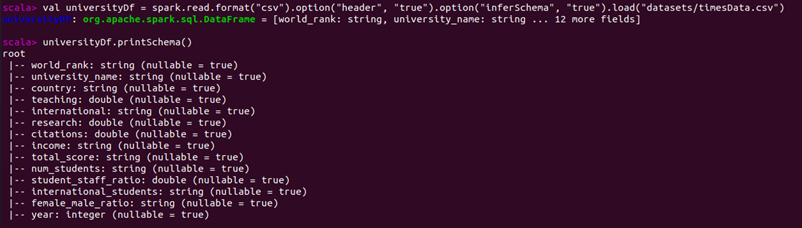
\includegraphics[width=\textwidth]{images/milepael5/csvRead.png}
\end{figure}

Jeg legger merke til at noen av datatypene ikke stemmer. Jeg ser at "world rank" er satt til streng, selv om det tilsynelatende er int. Men det går fin, siden den også inneholder verdier som "100 150". Derimot, "international" var satt til streng, fordi null-verdier var byttet ut med bindestrek , I tillegg så jeg at "international students" hadde verdier med tall og prosent-tegnet. Begge fikset jeg ved å bruke find and replace funksjonen i libreOffice og endre på csv-filen.

Da brukte jeg universityDf.printSchema() igjen for å sjekke at ting stemte, og det gjorde det.
\FigureCounter
\begin{figure}[H]
    
\includegraphics[width=\textwidth]{images/milepael5/printSchema.png}
\end{figure}

Det neste er å lagre den som en Parquet fil
\FigureCounter
\begin{figure}[H]
    
\includegraphics[width=\textwidth]{images/milepael5/writeParquet.png}
\end{figure}

\subsection{Første Aggregering}
Den første aggregeringen jeg lagde viser de ti skolene med flest kvinnelige studenter. 

\FigureCounter
\begin{figure}[H]
    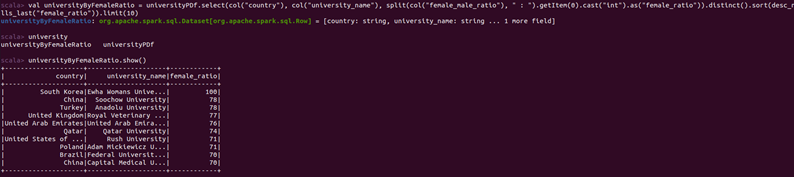
\includegraphics[width=\textwidth]{images/milepael5/uniFemaleRatio.png}
\end{figure}
\FigureCounter
\begin{figure}[H]
    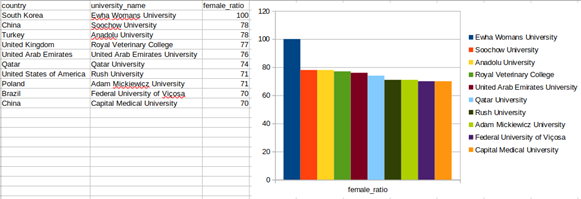
\includegraphics[width=\textwidth]{images/milepael5/resUniFemRatio.png}
\end{figure}

\subsection{Andre Aggregering}
Denne er tilsvarende forrige aggregering, men denne gangen for mannlige studenter.

\FigureCounter
\begin{figure}[H]
    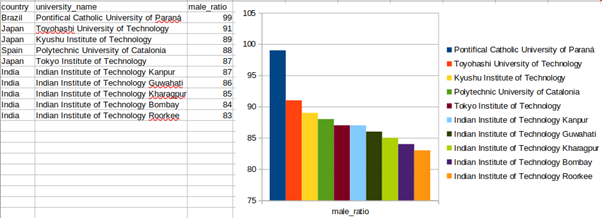
\includegraphics[width=\textwidth]{images/milepael5/resUniMaleRatio.png}
\end{figure}

Så lagret jeg begge aggregeringene som CSV filer med én partisjon hver.

\FigureCounter
\begin{figure}[H]
    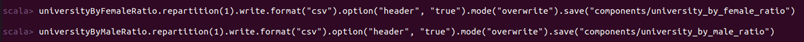
\includegraphics[width=\textwidth]{images/milepael5/writeToFile.png}
\end{figure}

\subsection{Tredje Aggregering}

Jeg lagde også en aggregering som viser gjennomsnitts-poeng per år. Denne var, til å begynne med, ment til å representere "Average Total Score by Number Of Students" komponentet fra forrige milepæl:

\FigureCounter
\begin{figure}[H]
    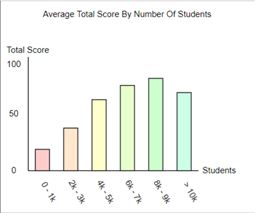
\includegraphics[width=\textwidth]{images/milepael5/avgScoreTotStudents.png}
\end{figure}

Her er den nye aggregeringen (Glemte å ta bilde av scala koden):

\FigureCounter
\begin{figure}[H]
    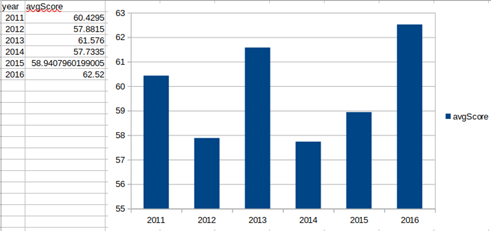
\includegraphics[width=\textwidth]{images/milepael5/avgScoreTotStudentsActual.png}
\end{figure}

